\section{Additional Data: The \texttt{phoneme} Dataset}\label{sec:additional-data}

The \texttt{phoneme} dataset, from the book \emph{Nonparametric Functional Data Analysis: Theory and Practice} by \textcite{ferraty_nonparametric_2006}\footnote{Data available at \url{https://www.math.univ-toulouse.fr/~ferraty/SOFTWARES/NPFDA/}.}, is a dataset from the field of speech recognition analysis.
It emanates from an original dataset used in the book \emph{The Elements of Statistical Learning} by \textcite{hastie_elements_2009}\footnote{Data available at \url{https://hastie.su.domains/ElemStatLearn/}.}.
The data contains observations of an audio signal that is transformed to the log-periodogram scale at a range of frequencies.
\textcite{ferraty_nonparametric_2006} provide $N=2000$ observations of the signal discretized onto a grid of $T=150$ equidistant frequencies, so that $\mathbf{X}$ is a $2000\times 150$ matrix containing the signals in its rows.
Figure \ref{fig:phoneme} displays a random sample of $8$ observations from the dataset.

\begin{figure}[h]
    \centering
    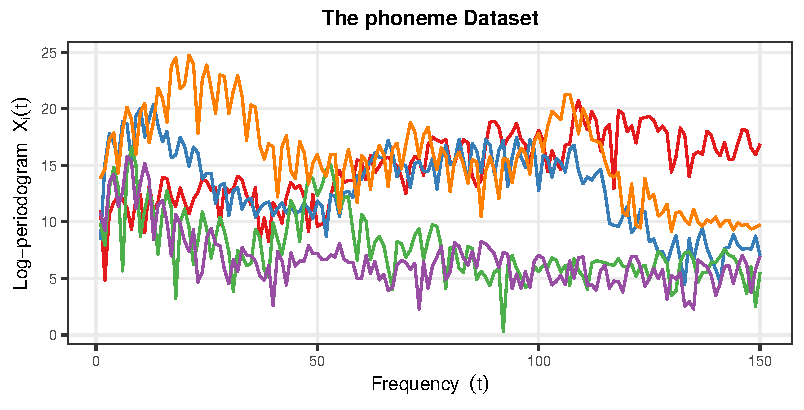
\includegraphics[width=0.75\linewidth]{figures/phoneme.pdf}
    \caption{A random sample of $8$ observations from the \texttt{phoneme} dataset \parencite{hastie_elements_2009, ferraty_nonparametric_2006}.}
    \label{fig:phoneme}
\end{figure}

